\documentclass{beamer}
\usepackage{hhline}
\usepackage[utf8]{inputenc}
\usepackage{subcaption}
\usepackage{placeins}
\usepackage{todonotes}
\usepackage{graphics}
\usepackage{graphicx,wrapfig,lipsum}


\usetheme{Copenhagen}

\title{
  Classification of ImageNet \\
  with Convolutional Neural Networks
}
\author{
  Niklas Lindqvist,\\
  Thony Price,\\
  William Skagerström\\
}

\begin{document}
\maketitle

\begin{frame}
  \frametitle{Agenda}

  \begin{itemize}
    \item Proposal and intention
    \item Implementation
    \item Results
  \end{itemize}
\end{frame}

\section{Proposal and intention}
\begin{frame}
  \frametitle{Project proposal}
  \begin{itemize}
	  \item Implement a CNN
    \item Achieve acceptable results in terms of accuracy (on ImageNet)
    \item Apply techniques from course to optimize performance of network
  \end{itemize}
\end{frame}

\section{Implementation}
\begin{frame}
  \frametitle{Research of the field}
  We began looking at state of the art
  \begin{itemize}
    \item GoogLeNet
    \item RezNet
    \item VGGNet
  \end{itemize}

  Then to more achievable en par with our scope. Here Stanford's course \textbf{CS231} proved a valuable source. There was many reports on classification of ImageNet by CNNs.
\end{frame}

\begin{frame}
  We went for an VGGNet inspired architecture of the network. The leftmost represents the most vanilla.
  \medskip

\begin{table}[htbp]
\begin{center}
\scalebox{0.6}{
\begin{tabular}{|c|c|c|c|}

  \hline
  \multicolumn{4}{|c|}{ConvNet Configuration} \\
  \hline

  A & B & C & D
  \\\hline

  SGD, RUI & Adam, RUI, BN &  Adam, RUI, Dropout & Adam, HEI, Dropout, BN
  \\\hhline{|=|=|=|=|}

  \multicolumn{4}{|c|}{input ($64\times64\times3\;RGB\;image$)}
  \\\hline

  conv-32, 2x2, ReLu & conv-32, 2x2, ReLu, BN & conv-32, 2x2, ReLu & conv-32, 2x2, ReLu, BN \\
  conv-32, 2x1, ReLu & conv-32, 2x1, ReLu, BN & conv-32, 2x1, ReLu & conv-32, 2x1, ReLu, BN \\
  conv-32, 1x2, ReLu & conv-32, 1x2, ReLu, BN & conv-32, 1x2, ReLu & conv-32, 1x2, ReLu, BN \\
  \hline
  MaxPooling, 2x2    & MaxPooling, 2x2    & MaxPooling, 2x2    & MaxPooling, 2x2 \\
  \hline
  conv-48, 2x2, ReLu & conv-48, 2x2, ReLu, BN & conv-48, 2x2, ReLu & conv-48, 2x2, ReLu, BN \\
  conv-48, 2x2, ReLu & conv-48, 2x2, ReLu, BN & conv-48, 2x2, ReLu & conv-48, 2x2, ReLu, BN \\
  conv-48, 2x2, ReLu & conv-48, 2x2, ReLu, BN & conv-48, 2x2, ReLu & conv-48, 2x2, ReLu, BN \\
  \hline
  MaxPooling, 2x2    & MaxPooling, 2x2    & MaxPooling, 2x2    & MaxPooling, 2x2 \\
  \hline
  conv-80, 2x2, ReLu & conv-80, 2x2, ReLu, BN & conv-80, 2x2, ReLu & conv-80, 2x2, ReLu, BN \\
  conv-80, 2x2, ReLu & conv-80, 2x2, ReLu, BN & conv-80, 2x2, ReLu & conv-80, 2x2, ReLu, BN \\
  conv-80, 2x2, ReLu & conv-80, 2x2, ReLu, BN & conv-80, 2x2, ReLu & conv-80, 2x2, ReLu, BN \\
  \hline
  MaxPooling, 2x2    & MaxPooling, 2x2        & MaxPooling, 2x2    & MaxPooling, 2x2 \\
  \hline
  FC-2048, ReLu      & FC-2048, ReLu, BN      & FC-2048, ReLu      & FC-2048, ReLu, BN
  \\\hline
  FC-200, SoftMax    & FC-200, SoftMax        & Dropout 0.3        & Dropout 0.3   \\
  \hline
                    &                         & FC-200, SoftMax    & FC-200, SoftMax \\
  \hline
  \end{tabular}
  }
% \caption[]
% {\small
%   Configuration of the four different CNNs tested initially. They differ in terms of solver (SGD/Adam), batch normalization (BN), Dropout and initializer (Random Unit Initialization/He Initialization).
% }
\label{table:3_configurations}
\end{center}
\end{table}

\end{frame}

\section{Results}
\begin{frame}
  We initialized a run on Google Cloud and the result was... OVERFITTING
\end{frame}



\begin{frame}
\centering
Network variant A
\begin{figure}[!h]
\centering
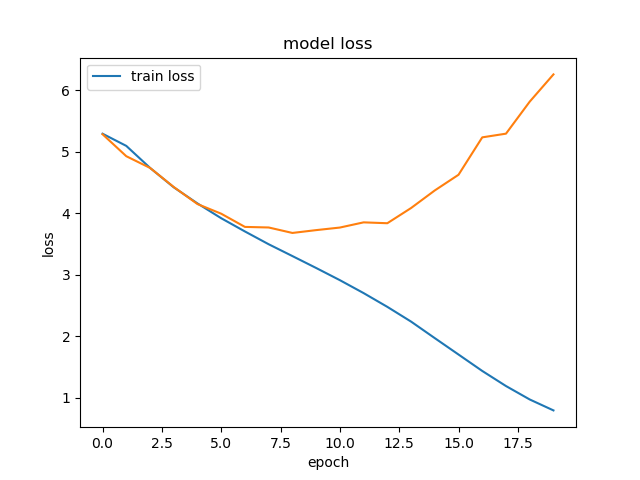
\includegraphics[width=0.7\textwidth]{images/run1_loss_a.png}
\end{figure}
\end{frame}

\begin{frame}
\centering
Network variant B
\begin{figure}[!h]
\centering
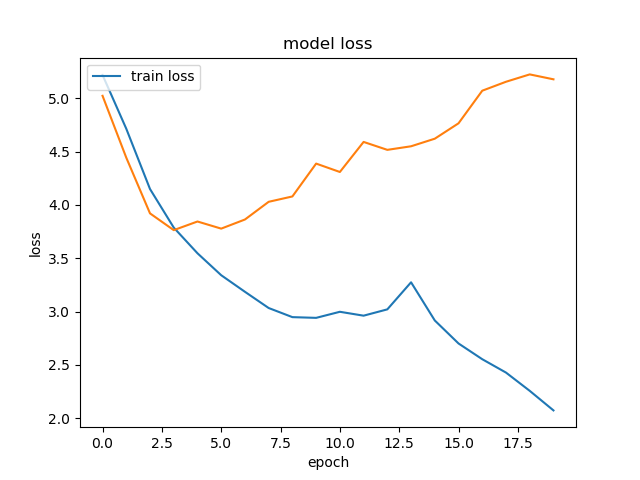
\includegraphics[width=0.7\textwidth]{images/run1_loss_b.png}
\end{figure}
\end{frame}

\begin{frame}
\centering
Network variant C
\begin{figure}[!h]
\centering
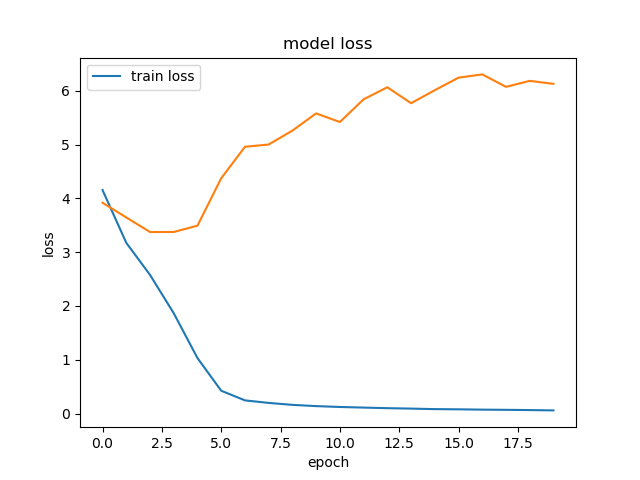
\includegraphics[width=0.7\textwidth]{images/run1_loss_c.png}
\end{figure}
\end{frame}

\begin{frame}
\centering
Network variant D
\begin{figure}[!h]
\centering
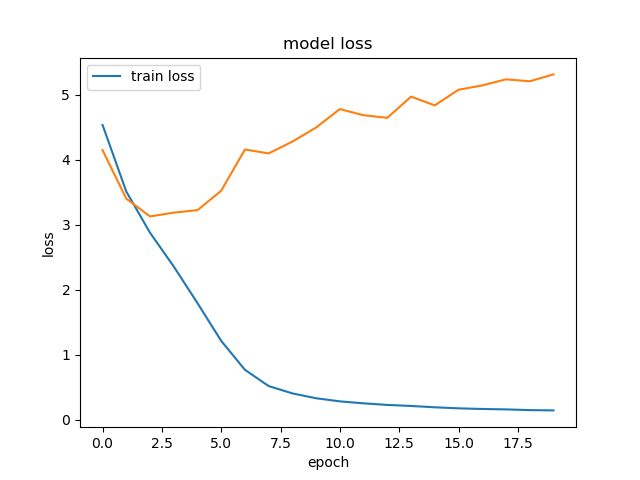
\includegraphics[width=0.7\textwidth]{images/run1_loss_d.png}
\end{figure}
\end{frame}




\begin{frame}
  To battle this we applied
  \begin{itemize}
    \item Batch normalization (All layers)
    \item Dropout (Dense layers)
    \item L2 regularization (X layers)
  \end{itemize}
  Tinkering with these variables resulted in improved performance \textbf{insert plot here/next slide}
\end{frame}




\end{document}

%\centering
%Network variant A (left) and B(right)
%\begin{figure}[!h]
%\centering
%\makebox[\textwidth]{
%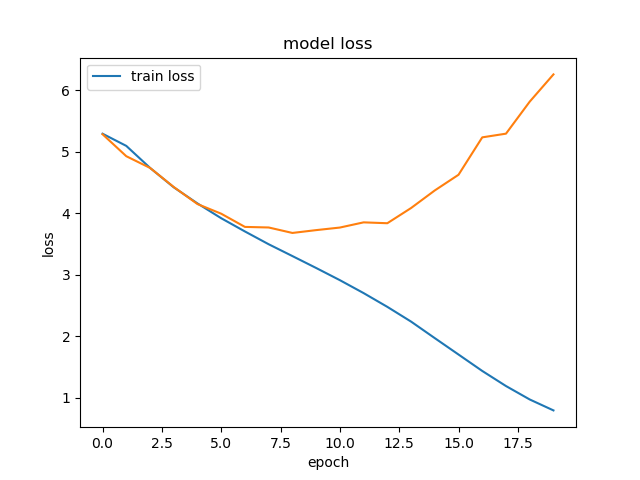
\includegraphics[width=0.3\textwidth]{images/run1_loss_a.png}
%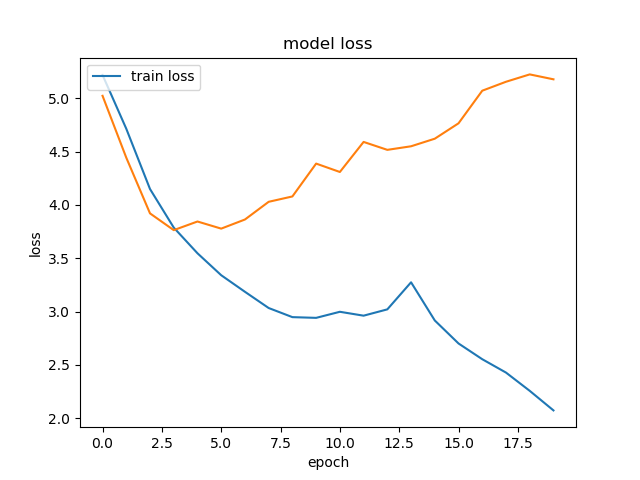
\includegraphics[width=0.3\textwidth]{images/run1_loss_b.png}
%}
%\end{figure}